
Let us define the basic model; our theoretical results admit some extensions, detailed in Section~\ref{sec:theory-extensions}.

\xhdr{Principals and agents.} There are two principals and $T$ agents,
denoted, resp., principal $i\in \{1,2\}$ and agent $t\in [T]$. The game proceeds in (global) rounds. In each round $t\in [T]$, the following  interaction takes place. Agent $t$ arrives and chooses a principal $i_t\in \{1,2\}$. The principal chooses action $a_t\in A$, where $A$ is a fixed set of actions (same for both principals and all rounds).%
\footnote{Throughout, we use `action' and `arm' interchangeably, as common in the literature on multi-armed bandits.}
 The agent experiences this action, receives a reward $r_t\in \{ 0,1\}$, and reports it back to the principal. We posit \emph{stochastic rewards}: whenever a given action $a\in A$ is chosen, the reward is an independent draw from Bernoulli distribution with mean $\mu_a$. The mean rewards $\mu_a$ are fixed over time, and initially not known to anybody. Each principal is completely unaware of the rounds when the other principal is chosen.

Each principal $i$ commits to a learning algorithm \alg[i] before round $1$, and uses this algorithm throughout. The algorithm follows the protocol of \emph{multi-armed bandits} (\emph{MAB}). Namely, it proceeds in time-steps:%
\footnote{These time-steps will sometimes be referred to as \emph{local steps/rounds}, so as to distinguish them from ``global rounds" defined before. We will omit the global vs. local distinction when clear from the context.} each time it is called, it outputs an action from $A$, and inputs a reward for this action. \alg[i] is called only in global rounds when principal $i$ is chosen.

\newcommand{\est}{\mathtt{EST}}

\xhdr{Agents' response.} Each agent $t$ forms a reward estimate $\est_i(t)\in [0,1]$ for each principal $i$, and chooses the principal based on these reward estimates. Specifically, principal $1$ is chosen with probability
\begin{align}
p_t = \respF\rbr{ \est_1(t) - \est_2(t) },
\end{align}
where $\respF:[-1,1]\to [0,1]$ is the \emph{response function}, same for all agents and known to everyone.

We assume that $\respF$ is monotonically non-decreasing, is larger than $\nicefrac12$ on the interval $(0,1]$, and smaller than $\nicefrac12$ on the interval $[-1,0)$. We consider three specific models (see \reffig{fig:response-functions}):

\begin{figure}
\begin{center}
  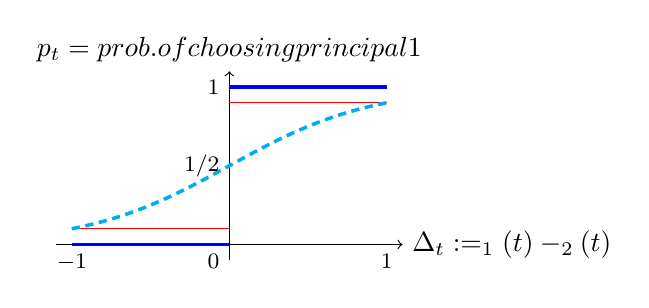
\begin{tikzpicture}[scale=2.0]
    \draw[->] (-1.1,0) -- (1.1,0) node[right]
    {$\Delta_t := \est_1(t) - \est_2(t)$};
    \draw[->] (0,-0.1) -- (0,1.1) node[above]
        {$p_t = \text{prob. of choosing principal 1}$};
    \draw[scale=1.0,domain=-1:0,smooth,variable=\q,blue, line width=0.50mm] plot ({\q},{0});
    \draw[scale=1.0,domain=0:1,smooth,variable=\q,blue,line width=0.50mm] plot ({\q},{1});
    \draw[scale=1.0,domain=-1:0,smooth,variable=\y,red]  plot ({\y},{0.1});
    \draw[scale=1.0,domain=0:1,smooth,variable=\y,red]  plot ({\y},{0.9});
    \draw[scale=1.0,domain=-1:1,smooth,variable=\y,cyan, line width=0.45mm, dash pattern=on 3pt off 2pt]  plot ({\y},{1/(1 + 1/(9^\y))});
    % \node[above, blue] at (0.5, 0.5) {\footnotesize $2 q (1 - q)$};
     \node[left] at (0, 0.5) {\footnotesize $1/2$};
     \node[left] at (0, 1) {\footnotesize $1$};
     \node[below left] at (0, 0) {\footnotesize $0$};
     \node[below ] at (1, 0) {\footnotesize $1$};
     \node[below ] at (-1, 0) {\footnotesize $-1$};
  \end{tikzpicture}
\end{center}
\caption{The three models for $\respF$: \HardMax is thick blue, \HardMaxRandom is slim red, and \SoftMaxRandom is the dashed curve.}
\label{fig:response-functions}
\end{figure}

\begin{itemize}
\item \HardMax: $\respF$ equals $0$ on the interval $[-1,0)$ and $1$
  on the interval $(0,1]$. In words, a \HardMax agent
  deterministically chooses a principal with a higher reward estimate.

\item \HardMaxRandom:
    % $\respF$ equals $\eps$ on the interval $[-1,0)$ and $1-\eps'$ on the interval $(0,1]$, where $\eps,\eps'\in (0,\tfrac12)$ are some positive constants. In words, each agent is a \HardMax agent with probability $1-\eps-\eps'$, and with the remaining probability she makes a random choice.
    $\respF$ equals $\eps_0$ on the interval $[-1,0)$ and $1-\eps_0$ on the interval $(0,1]$, for some constant $\eps_0\in (0,\tfrac12)$. In words, each agent is a \HardMax agent with probability $1-2\eps_0$, and makes a random choice otherwise.


\item \SoftMaxRandom: $\respF(\cdot)$ is bounded away from $0$ and $1$, and ``smooth" around $0$ (see Section~\ref{sec:theory-SoftMax}).
\end{itemize}
% \asedit{(We assume $\respF(-1)+\respF(1)=1$ in \HardMaxRandom and \SoftMaxRandom only to simplify notation.)}


%We say that $\respF$ is \emph{symmetric} if $\respF(-x)+\respF(x)=1$ for any $x\in [0,1]$. This implies \emph{fair tie-breaking}: $\respF(0)=\tfrac12$.

\xhdr{Bayesian vs. frequentist.}
We consider two model variants, Bayesian and frequentist. The main difference between the two concerns the agents' reward estimates $\est_i(t)$.

\begin{itemize}
\item In the \emph{\TheoryModel}, the mean reward vector $\mu = (\mu_a:\; a\in A)$ is drawn from a common Bayesian prior $\priorMu$. Agents know the principals' algorithms. Their reward estimates are defined as posterior mean rewards:
        $\est_i(t) = \PMR_i(t) := \E\sbr{ r_t\mid i_t = i }$
    for each agent $t$ and principal $i$.

\item In the \emph{\ExptsModel}, agents' reward estimate for a given principal is the average reward of the last $M$ agents that chose this principal (interpreted as a \emph{reputation score}). To make the reputation score meaningful initially, each principal enjoys a ``warm start": additional $T_0$ agents arrive before the game starts, and interact with the principal as described above.

\end{itemize}

\xhdr{Competition game.}
Some of our results explicitly study the game between the two principals, termed the \emph{competition game}. We model it as a simultaneous-move game: before the first agent arrives, each principal commits to an MAB algorithm. Thus, choosing a pure strategy in this game corresponds to choosing an MAB algorithm. Principal's utility is defined as the market share, \ie the number of agents that chose this principal. Principals are risk-neutral, in the sense that they optimize their expected utility.

